\chapter{Implementation}
In this section we will discuss the implementation of our previously discussed design. More specifically, the electronic hardware and software systems.

\section{Hardware implementation}
The hardware systems are implemented using two printed circuit boards (PCBs), one for each microcontroller. These handle the communication between the microcontrollers and the execution of actions, requested by the control device laptop.

\subsection{Printed Circuit Boards}

The first PCB is for the PIC18F slave microcontroller. The PIC18F resides in the middle and is the central unit of this board. The PCB contains a connection for the solenoid, to control when it need to turn on and off. It also contains connections for the servo motor and its control circuit which is a simple MOSFET transistor circuit. The board also contains connections for the NRF24 module, to make radio communication with the ESP32 possible. This PCB design can be seen in Figure~\ref{fig:pic-pcb}.

\begin{figure}[h]
	\centering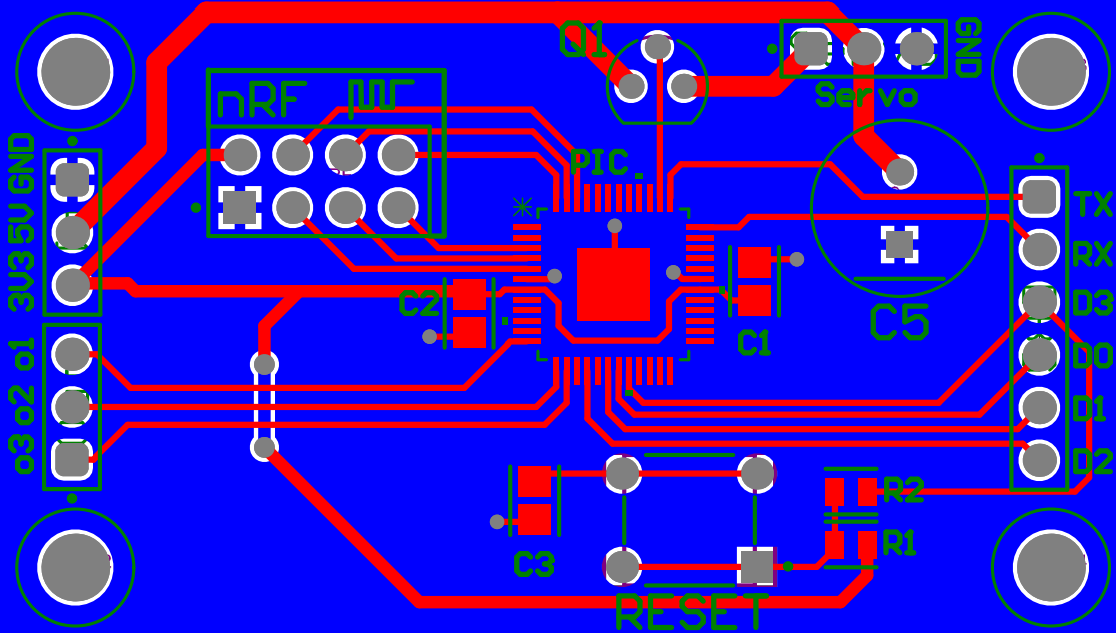
\includegraphics[height=5cm]{./images/PIC18F_pcb}
	\caption{PIC18F PCB Design}
	\label{fig:pic-pcb}
\end{figure}

The second PCB is for the ESP32 master controller. This PCB consists of pin headers for the ESP32 controller itself, and pin headers for each of the DRV8825 modules, which control the stepper motors. It has switches for on board adjustment of the drivers' control pins. It also contains connections for the NRF24 module, like the PIC18F. This PCB design can be seen in Figure~\ref{fig:esp-pcb}. 

\begin{figure}[h]
	\centering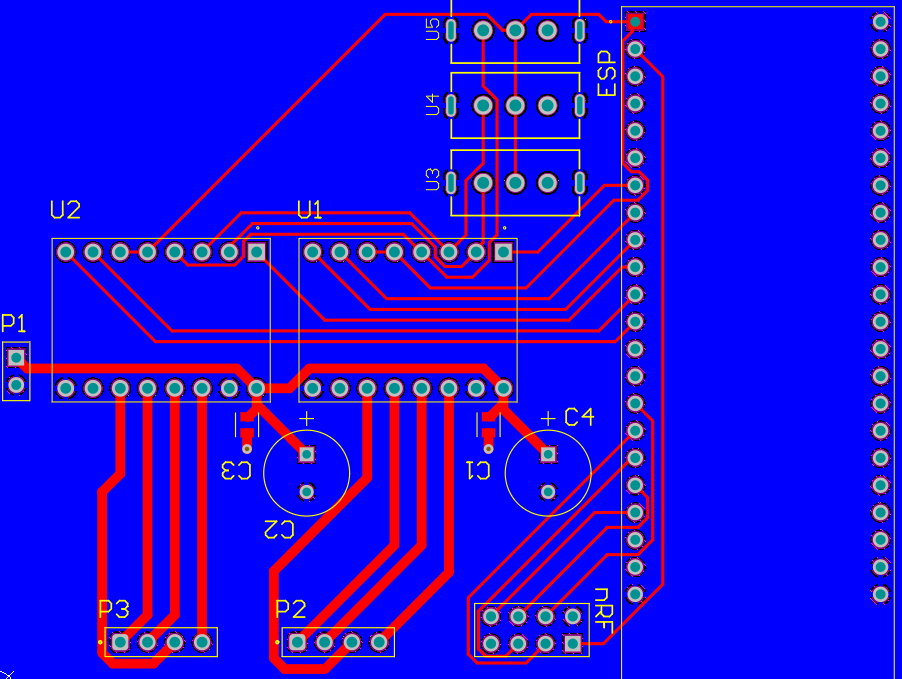
\includegraphics[height=5cm]{./images/ESP32_pcb}
	\caption{ESP32 PCB Design}
	\label{fig:esp-pcb}
\end{figure}


\section{Software implementation}

The embedded software system is developed for an ESP32-based real-time application involving motion control and wireless communication. The design follows a modular, task-based architecture utilizing the FreeRTOS operating system, allowing concurrent execution of multiple subsystems and ensuring responsiveness to real-time events.

\subsection{Architectural Overview}
The system architecture is composed of three primary subsystems: a communication subsystem, a motion control subsystem, and a simulation/testing subsystem. These subsystems interact through well-defined interfaces and communicate via FreeRTOS message queues, allowing asynchronous data exchange and decoupling between components.

\subsection{Communication Subsystem}
The communication subsystem is responsible for receiving external control commands via UDP over Wi-Fi and transmitting actuator signals through an NRF24 radio interface. The UDP client manages socket creation, data reception, and error handling, converting received commands into structured messages. These messages are placed into dedicated queues for consumption by the motion and actuator controllers. The NRF24-based radio communication provides an additional, low-latency communication channel for controlling remote actuators, contributing to the system's flexibility and scalability.

\subsection{Motion Control Subsystem}
The motion control subsystem handles the operation of two stepper motors along orthogonal axes. Motor control is implemented using hardware timers configured to trigger interrupts at precise intervals. Within the interrupt service routines, step signals are toggled, positions are updated, and step frequencies are adjusted according to desired momentum and target positions. The use of easing functions ensures smooth acceleration and deceleration, minimizing mechanical stress and enabling precise control. Position and speed adjustments are driven by messages received from the communication subsystem, allowing dynamic and responsive actuation.

\subsection{Simulation and Testing Subsystem}
To facilitate development and validation in the absence of hardware, the system incorporates a simulation and testing subsystem. Mock tasks generate synthetic messages simulating both UDP communication and actuator commands. This feature enables rigorous testing of system behavior, ensuring robustness and correctness prior to hardware deployment.

\subsection{Inter-task Communication and Decoupling}
The system employs three dedicated message queues for horizontal stepper control, vertical stepper control, and racket actuator commands. These queues enable asynchronous, thread-safe communication between tasks. The use of structured message formats for stepper and actuator commands maintains consistency and simplifies message handling logic, supporting scalability and modular expansion.

\subsection{Modularity and Configurability}
The firmware includes compile-time configuration flags to enable or disable subsystems such as UDP communication, radio communication, stepper control, and mock simulation tasks. This configurability allows the firmware to be adapted for various development and deployment scenarios, including partial module testing, hardware-in-the-loop simulations, or full production operation.

\subsection{Design Rationale}
The overall system design reflects a deliberate emphasis on separation of concerns, real-time responsiveness, scalability, and testability. The modular task-based architecture and asynchronous queue-based messaging enable the system to maintain predictable real-time behavior while remaining adaptable to future expansions or modifications. The inclusion of simulation capabilities addresses the need for verification and debugging in complex embedded systems where hardware access may be limited during certain development phases.

\subsection{Conclusion}
In conclusion, the software architecture presented here demonstrates an effective approach for real-time motion control and communication in an embedded environment. Through its modular design, task-based concurrency, and flexible configuration, the system achieves a balance between robustness, maintainability, and adaptability, making it well-suited for both research and applied deployment in embedded control scenarios.